\documentclass{article}
% Set operations illustrated with Venn diagrams
% Author: Uwe Ziegenhagen
% This is an expanded version of an example provided by T. Tantau

\usepackage{tikz}
\usepackage{pgfplots}
\usepackage{amsmath}
%%%<
\usepackage{verbatim}
%\usepackage[active,tightpage]{preview}
\usetikzlibrary{shapes,decorations,plotmarks,snakes,decorations.markings,intersections}
%\PreviewEnvironment{tikzpicture}
%\setlength\PreviewBorder{5pt}%
%%%>

%%
%% CALCIUM DEFINITIONS   
%%

% My Definitions

\def\FcepsilonR1{Fc$\epsilon$R1}

\def\Ps{$\ps$}
\def\ps{{\rm s}^{-1}}

\def\Pms{$\pms$}
\def\pms{{\rm ms}^{-1}}

\def\UM{$\uM$}
\def\uM{\mu{\rm M}}

\def\Um{$\um$}
\def\um{\mu{\rm m}}

\def\Us{$\us$}
\def\us{\mu{\rm s}}

\def\Ums{$\ums$}
\def\ums{\mu{\rm m}^2}

\def\Nm{$\nm$}
\def\nm{\mu{\rm m}}

\def\Pumps{$\pumps$}
\def\pumps{\mu{\rm M}^{-1} {\rm s}^{-1}}

\def\Pumpms{$\pumpms$}
\def\pumpms{\mu{\rm M}^{-1} {\rm ms}^{-1}}

\def\UMps{$\uMps$}
\def\uMps{\mu{\rm M}/{\rm s}}

\def\Umpss{$\umpss$}
\def\umpss{\mu{\rm m}/{\rm s}^2}

\def\Umsps{$\umsps$}
\def\umsps{\mu{\rm m}^2/{\rm s}}

\def\Umspms{$\umspms$}
\def\umspms{\mu{\rm m}^2/{\rm ms}}

\def\Ryr{RyR}
\def\ip{{[{\rm IP}_3]}}

\def\Ip{${\rm IP}_3$}
\def\Ipr{${\rm IP}_3{\rm R}$}

\def\cad{[{\rm Ca}^{\rm 2+}]_{\rm d}}
\def\Cad{$\cad$}

\def\cabulk{[{\rm Ca}^{\rm 2+}]_{\rm bulk}}
\def\Cabulk{$\cabulk$}

\def\cainf{[{\rm Ca}^{\rm 2+}]_{\infty}}
\def\Cainf{$\cainf$}

\def\cai{[{\rm Ca}^{\rm 2+}]_{\rm i}}
\def\Cai{$\cai$}

\def\caext{[{\rm Ca}^{\rm 2+}]_{\rm ext}}
\def\Caext{$\caext$}

\def\cae{[{\rm Ca}^{\rm 2+}]_{\rm ER}}
\def\Cae{$\cae$}

\def\cat{[{\rm Ca}^{\rm 2+}]_{\rm T}}
\def\Cat{$\cat$}

\def\ve{{\varepsilon}}
\def\Bj{${\rm B}_j$}
\def\B{${\rm B}$}
\def\Bt{$\bt$}
\def\Ca{${\rm Ca}^{\rm 2+}$}
\def\K{${K}^{+}$}
\def\Cabj{${\rm CaB}_j$}
\def\Cab{${\rm CaB}$}
\def\Kj{$\kj$}
\def\Kjm{$\kjm$}
\def\Kjp{$\kjp$}
\def\Kmm{$\kmm$}
\def\Kkm{$\kkm$}
\def\Kmp{$\kmp$}
\def\Km{$\km$}
\def\Kp{$\kp$}
\def\bjt{\bj_T}
\def\b{[{\rm B}]}
\def\bj{[{\rm B}_j]}
\def\bmt{\bm_T}
\def\bt{\b_{\rm T}}
\def\bm{[B_m]}
\def\cabj{[{\rm CaB}_j]}
\def\cab{[{\rm CaB}]}
\def\ca{[{\rm Ca}^{2+}]}
\def\dc{D_c}
\def\dj{D_j}
\def\dm{D_m}
\def\db{D_b}
\def\kj{K_j}
\def\kjm{k^-_j}
\def\kjp{k^+_j}
\def\kmm{k^-_m}
\def\kmp{k^+_m}
\def\kkm{K_m}
\def\km{k^-}
\def\kp{k^+}

\def\wm{w^-}
\def\wp{w^+}
\def\minf{m_\infty}

% other ions

\def\mg{[{\rm Mg}^{2+}]}
\def\Mg{${\rm Mg}^{\rm 2+}$}




%%
%% MATH DEFINITIONS   
%%

\def\({\left(}
\def\){\right)}

\def\inv#1{{\frac{1}{#1}}}
\def\ddt#1{\der{#1}{t}}
\def\ddx#1{\der{#1}{x}}
\def\ddz#1{\der{#1}{z}}
\def\der#1#2{{\frac{d#1}{d#2}}}
\def\derder#1#2{{d^2\frac{#1}{d{#2}^2}}}
\def\norm#1{\labs #1 \rabs}
\def\pder#1#2{{\frac{\partial#1}{\partial#2}}}
\def\pderder#1#2{{\frac{\partial^2#1}{\partial{#2}^2}}}
\def\pdt#1{\pder{#1}{t}}
\def\pdx#1{\pder{#1}{x}}
\def\pdxx#1{\pderder{#1}{x}}
\def\pdz#1{\pder{#1}{z}}
\def\pdzz#1{\pderder{#1}{z}}
\def\ssize#1{{\scriptsize #1}}

\def\bmat{\left[ \begin{array}}
\def\bna{\begin{array}}
\def\bneas{\begin{eqnarray*}}
\def\bnea{\begin{eqnarray}}
\def\bnes{\begin{displaymath}}
\def\bne{\begin{equation}}

\def\emat{\end{array} \right]}
\def\ena{\end{array}}
\def\eneas{\end{eqnarray*}}
\def\enea{\end{eqnarray}}
\def\enes{\end{displaymath}}
\def\ene{\end{equation}} 

\def\half{\frac{1}{2}} 

\def\revrxn#1#2{
\begin{array}{c} 
{#1}\\
\rightleftharpoons \\
{#2}
\end{array}
}

\def\Bold#1{\vspace{0.1in} \noindent {\bf \boldmath #1}}

\def\Sec#1{Section~\ref{#1}}
\def\Secs#1#2{Sections~\ref{#1}--\ref{#2}}
\def\SecsAnd#1#2{Sections~\ref{#1} and \ref{#2}}

\def\Eqn#1{Eq.~\ref{#1}}
\def\Eqns#1#2{Eqs.~\ref{#1}--\ref{#2}}
\def\EqnsAnd#1#2{Eqs.~\ref{#1} and \ref{#2}}

\def\Eq#1{Eq.~\ref{#1}}
\def\Eqs#1#2{Eqs.~\ref{#1}--\ref{#2}}
\def\EqsAnd#1#2{Eqs.~\ref{#1} and \ref{#2}}

\def\Fig#1{Fig.~\ref{#1}}
\def\Figs#1#2{Figs.~\ref{#1}--\ref{#2}}
\def\FigsAnd#1#2{Figs.~\ref{#1} and \ref{#2}}

\def\Figure#1{Figure~\ref{#1}}
\def\Figures#1#2{Figures~\ref{#1}--\ref{#2}}
\def\FiguresAnd#1#2{Figures~\ref{#1} and \ref{#2}}

\def\avg#1{\langle{#1}\rangle}
\def\Parens#1{\left({#1}\right)}

\def\Bold#1{{\bf #1}}
\def\Block#1#2{{\bf #1:} {#2}\\ }

\def\bfcite#1{{\bf\cite{#1}}}

\def\bpi{\boldsymbol \pi}
\def\E{\mathsf E}
\def\P{\mathsf P}
\def\Pr{\mathsf P}
\def\Var{\mathsf{Var}}



% in math mode include brackets 
\def\ca{[{\rm Ca}^{2+}]} 
\def\na{[{\rm Na}^{+}]}
\def\k{{[\rm K}^{+}]}
\def\cl{[{\rm Cl}^{-}]}

% but in text mode don't include brackets 
\def\Ca{${\rm Ca}^{2+}$} 
\def\Na{${\rm Na}^{+}$}
\def\K{${\rm K}^{+}$}
\def\Cl{${\rm Cl}^{-}$}

\def\ica{I_{\rm Ca}}
\def\ina{I_{\rm Na}}
\def\ik{I_{\rm K}}
\def\ikca{I_{\rm K-Ca}}
\def\ikdr{I_{\rm K-DR}}
\def\ia{I_{\rm A}}
\def\icl{I_{\rm Cl}}
\def\iapp{I_{\rm app}}
\def\iadap{I_{\rm adap}}
\def\il{I_{\rm L}}
%Can't use \it because it means italic! 
\def\iit{I_{\rm T}}
\def\ih{I_{\rm h}}

\def\Ica{$\ica$}
\def\Ina{$\ina$}
\def\Ik{$\ik$}
\def\Ikca{$\ikca$}
\def\Ikdr{$\ikdr$}
\def\Ia{$\ia$}
\def\Icl{$\icl$}
\def\Il{$\il$}
\def\It{$\iit$}
\def\Ih{$\ih$}
\def\Iapp{$\iapp$}
\def\Iadap{$\iadap$}

\def\gca{g_{\rm Ca}}
\def\gna{g_{\rm Na}}
\def\gk{g_{\rm K}}
\def\ga{g_{\rm A}}
\def\gcl{g_{\rm Cl}}
\def\gl{g_{\rm L}}
\def\gt{g_{\rm T}}
\def\gh{g_{\rm h}}
\def\gadap{g_{\rm adap}}

\def\gcabar{\bar{g}_{\rm Ca}}
\def\gnabar{\bar{g}_{\rm Na}}
\def\gkbar{\bar{g}_{\rm K}}
\def\gclbar{\bar{g}_{\rm Cl}}

\def\Gca{$\gca$} 
\def\Gna{$\gna$} 
\def\Gk{$\gk$} 
\def\Ga{$\ga$} 
\def\Gcl{$\gcl$}
\def\Gl{$\gl$}
\def\Gt{$\gt$}
\def\Gh{$\gh$}
\def\Gadap{$\gadap$}

\def\Gcabar{$\gcabar$} 
\def\Gnabar{$\gnabar$} 
\def\Gkbar{$\gkbar$} 
\def\Gclbar{$\gclbar$}

\def\eca{E_{\rm Ca}}
\def\ena{E_{\rm Na}}
\def\ek{E_{\rm K}}
\def\ecl{E_{\rm Cl}}
\def\el{E_{\rm L}}

\def\Eca{$\eca$} 
\def\Ena{$\ena$} 
\def\Ek{$\ek$} 
\def\Ecl{$\ecl$}
\def\El{$\el$}

\def\vca{V_{\rm Ca}}
\def\vna{V_{\rm Na}}
\def\vk{V_{\rm K}}
\def\vcl{V_{\rm Cl}}
\def\vl{V_{\rm L}}
\def\vt{V_{\rm T}}

\def\Vca{$\vca$} 
\def\Vna{$\vna$} 
\def\Vk{$\vk$} 
\def\Vcl{$\vcl$}
\def\Vl{$\vl$}
\def\Vt{$\vt$}

\def\Kir{$K_{\rm ir}$}






% The data files, written on the first run.
\begin{filecontents}{div_soft.data}
#MOPS 	Power [mW]
1.33E-02	10.403432
1.33E-01	12.53108
2.66E-01	14.90265
3.99E-01	17.22483
5.31E-01	19.58292
6.64E-01	21.89876
7.97E-01	24.44624
9.30E-01	26.6708
\end{filecontents}

\begin{filecontents}{div_ciu.data}
# MOPS 	Power [mW]
4.35E-02	9.562436
4.35E-01	10.845494
8.69E-01	12.24356
1.30E+00	13.66974
1.74E+00	15.13008
2.17E+00	16.57845
2.61E+00	17.97894
3.04E+00	19.41534
\end{filecontents}

\begin{filecontents}{div_ciu_oscar.data}
#MOPS 	Power [mW]
8.57E-01	11.255013
9.99E-01	11.4804
1.14E+00	11.718
1.29E+00	11.9916
1.64E+00	12.65854
2.00E+00	13.308
2.64E+00	14.484
3.85E+00	16.8
\end{filecontents}

\begin{filecontents}{div_ciu_oscar_extrapolated.data}
# MOPS 	Power [mW]
4.28E+00	17.56312023
5.71E+00	20.21127914
7.14E+00	22.85943805
8.57E+00	25.50759696
9.99E+00	28.15575587
\end{filecontents}

\begin{filecontents}{characteristic_time_sigmoid.data}

\end{filecontents}


\begin{document}
% multiple ECG traces (trying to get sampling to work).
\begin{figure}[t] 
\begin{center}
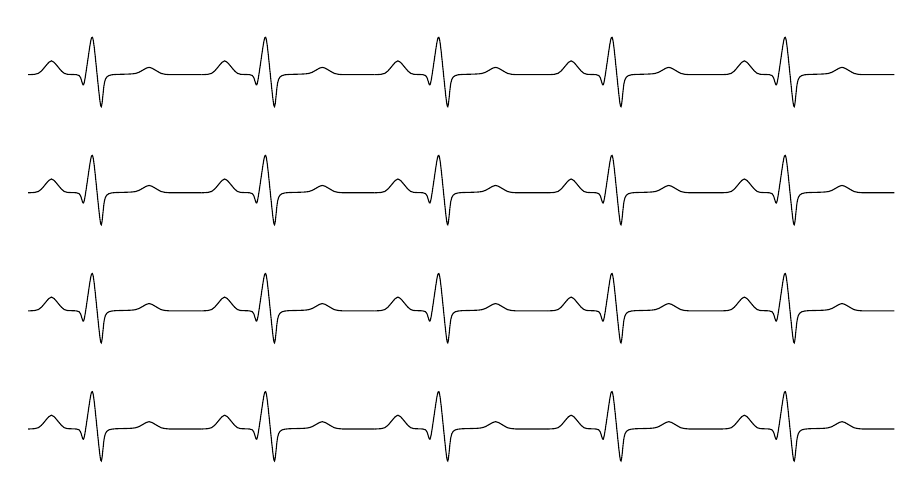
\begin{tikzpicture}[scale=0.5]
\foreach \yshift in { 0, 3, 6, 9} {
\foreach \x in { 0, 4.40,8.80,13.20,17.60} {
\begin{scope}[xshift=\x cm,yshift=\yshift cm]
\draw (0,0) .. controls (.27,.01) .. ({(.27+.59)/2},{(.01+.40)/2})
					.. controls  (.59,.40) .. ({(.59+.91)/2},{(.40+.01)/2})
					.. controls (.91,.01) .. ({(.91+1.31)/2},{(.01+0)/2})
					.. controls (1.31,0) .. ({(1.31+1.41)/2},{(0+-.34)/2})
					.. controls (1.41,-.34) .. ({(1.41+1.63)/2},{(-.34+1.18)/2})
					.. controls (1.63,1.18) .. ({(1.63+1.85)/2},{(1.18+-0.99)/2})
					.. controls  (1.85,-0.99) .. ({(1.85+1.95)/2},{(-0.99+0)/2})
					.. controls (1.95,0) .. ({(1.95+2.75)/2},{(0+.02)/2})
					.. controls (2.75,.02) .. ({(2.75+3.07)/2},{(.02+.21)/2})
					.. controls (3.07,.21) .. ({(3.07+3.39)/2},{(.21+.02)/2})
					.. controls (3.39,.02) .. ({(3.39+3.57)/2},{(.02+0)/2})
					.. controls (3.57,0) .. ({(3.57+3.90)/2},{(0+0)/2})
					.. controls (3.90,0) .. (4.40,0); 

%\foreach \w in {0,1,2,3,4,5,6,7,8,9,10}				
%\fill[white] (0.2*\w,-1) rectangle (0.2*\w+0.1,1);

\end{scope}
}
}
\end{tikzpicture}
\end{center}
\caption{Sampling with a time step similar to (or longer than) characteristic time may obscure the important features of a biological signal. }
\end{figure}


\clearpage


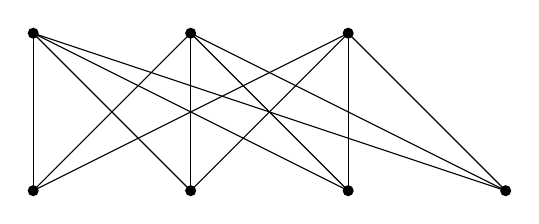
\begin{tikzpicture}[scale=2]
   \foreach \i in {1,...,4}
   {
      \path (\i,0) coordinate (X\i);
      \fill (X\i) circle (1pt);
   }
   \foreach \j in {1,...,3}
   {
      \path (\j,1) coordinate (Y\j);
      \fill (Y\j) circle (1pt);
   }
   \foreach \i in {1,...,4}
   {
      \foreach \j in {1,...,3}
      {
         \draw (X\i) -- (Y\j);
      }
   }
\end{tikzpicture}

\clearpage




\begin{tikzpicture}[y=.2cm, x=.7cm,font=\sffamily]
 	%axis
	\draw (0,0) -- coordinate (x axis mid) (10,0);
    	\draw (0,0) -- coordinate (y axis mid) (0,30);
    	%ticks
    	\foreach \x in {0,...,10}
     		\draw (\x,1pt) -- (\x,-3pt)
			node[anchor=north] {\x};
    	\foreach \y in {0,5,...,30}
     		\draw (1pt,\y) -- (-3pt,\y) 
     			node[anchor=east] {\y}; 
	%labels      
	\node[below=0.8cm] at (x axis mid) {MOPS};
	\node[rotate=90, above=0.8cm] at (y axis mid) {Power [mW]};

	%plots
	\draw plot[mark=*, mark options={fill=white}] 
		file {div_soft.data};
	\draw plot[mark=triangle*, mark options={fill=white} ] 
		file {div_ciu.data};
	\draw plot[mark=square*, mark options={fill=white}]
		file {div_ciu_oscar.data};
	\draw plot[mark=square*]
		file {div_ciu_oscar_extrapolated.data};  
    
	%legend
	\begin{scope}[shift={(4,4)}] 
	\draw (0,0) -- 
		plot[mark=*, mark options={fill=white}] (0.25,0) -- (0.5,0) 
		node[right]{soft};
	\draw[yshift=\baselineskip] (0,0) -- 
		plot[mark=triangle*, mark options={fill=white}] (0.25,0) -- (0.5,0)
		node[right]{ciu};
	\draw[yshift=2\baselineskip] (0,0) -- 
		plot[mark=square*, mark options={fill=white}] (0.25,0) -- (0.5,0)
		node[right]{ciu + oscar};
	\draw[yshift=3\baselineskip] (0,0) -- 
		plot[mark=square*, mark options={fill=black}] (0.25,0) -- (0.5,0)
		node[right]{ciu + oscar extrapolated};
	\end{scope}
\end{tikzpicture}




% exponential relaxation
\def\tmax{12}
\def\tmin{-1}
\def\tcm{6}
\def\tscale{\tcm/(\tmax-\tmin)}
\def\xmax{12}
\def\xmin{-1}
\def\xcm{5}
\def\xscale{\xcm/(\xmax-\xmin)}
\def\ticklen{1.5} % in units of t
\def\xinit{9}
\def\xinf{5}
\def\taux{6}
\begin{figure}
\begin{tikzpicture}[xscale=\tscale,yscale=\xscale]
\draw[thick,->] (\tmin,0) -- (\tmax,0) node[below left] {$t$};
\draw[thick,->] (0,\xmin) -- (0,\xmax) node[below left] {$x(t)$} node [below right] {$= x_\infty + \underbrace{\left( x_0 - x_\infty \right)}_{\mbox{positive}} \exp(-t/\tau)$};
\draw[blue, ultra thick, domain=0:\tmax] plot (\x, {(\xinit-\xinf)*exp(-\x/\taux)+\xinf}) [->];
\draw[dotted, thick] (0,\xinf) --  (\tmax, \xinf);
\draw[thick,|->|,inner sep=5pt]  (-2ex,\xinf) node[left] {$x_\infty$} --  (-2ex,\xinit) node[left] {$x_0$}; 

\begin{scope}[xshift=\taux cm]
\draw[thick, dotted]  (0,-\ticklen/4) node[below] {$\tau$} -- (0,\xinf) node[below] {}; 
\draw[thick,|->]  (0,\xinf) node[below] {} -- node[left] {$(x_0-x_\infty)/e$} (0,{(\xinit-\xinf)/exp(1)+\xinf}) node[above] {$x(\tau)$}; 
\end{scope}

\def\xinit{1}
\begin{scope}[xshift=15cm]
\draw[thick,->] (\tmin,0) -- (\tmax,0) node[below left] {$t$};
\draw[thick,->] (0,\xmin) -- (0,\xmax) node[below left] {$x(t)$} node [below right] {$= x_\infty + \underbrace{\left( x_0 - x_\infty \right)}_{\mbox{negative}}  \exp(-t/\tau)$};

\draw[dotted, thick] (0,\xinf) --  (\tmax, \xinf);
\draw[thick,|->|,inner sep=5pt]  (-2ex,\xinf) node[left] {$x_\infty$} --   (-2ex,\xinit) node[left] {$x_0$}; 

\begin{scope}[xshift=\taux cm]
\draw[thick, dotted]  (0,-\ticklen/4) node[below] {$\tau$} -- (0,\xinf) node[below] {}; 
\draw[thick,|->]  (0,\xinf) node[below] {} -- node[left] {$(x_0-x_\infty)/e$} (0,{(\xinit-\xinf)/exp(1)+\xinf}) node[below,fill=white] {$x(\tau)$}; 
\end{scope}

\draw[blue, ultra thick, domain=0:\tmax] plot (\x, {(\xinit-\xinf)*exp(-\x/\taux)+\xinf}) [->];

\end{scope}
\end{tikzpicture}
\caption{Exponential relaxation.}
\end{figure}




% exponential relaxation
\def\tmax{12}
\def\tmin{-1}
\def\tcm{6}
\def\tscale{\tcm/(\tmax-\tmin)}
\def\xmax{12}
\def\xmin{-1}
\def\xcm{5}
\def\xscale{\xcm/(\xmax-\xmin)}
\def\ticklen{1.5} % in units of t
\def\xinit{9}
\def\xinf{5}
\def\taux{6}
\begin{figure}
\begin{tikzpicture}[xscale=\tscale,yscale=\xscale]

\draw[thick,->] (\tmin,0) -- (\tmax,0) node[below left] {$t$};
\draw[thick,->] (0,\xmin) -- (0,\xmax) node[below left] {$x(t)$} node [below right] {$= x_\infty + \underbrace{\left( \{ x_0 \} - x_\infty \right)}_{\mbox{positive}} \exp(-t/\tau)$};
\foreach \xinitscale in {0.25, 0.5, 1} {
\draw[blue, ultra thick, domain=0:\tmax,samples=100] plot (\x, {\xinitscale*(\xinit-\xinf)*exp(-\x/\taux)+\xinf}) [->];
\draw[thick,|->|,inner sep=5pt]  (-2ex,\xinf) node[left] {$x_\infty$} --  (-2ex,{\xinitscale*(\xinit-\xinf)+\xinf}) node[left] {$x_0$}; 
}
\draw[dotted, thick] (0,\xinf) --  (\tmax, \xinf);


\begin{scope}[xshift=15cm]
\def\xinit{1}
\draw[thick,->] (\tmin,0) -- (\tmax,0) node[below left] {$t$};
\draw[thick,->] (0,\xmin) -- (0,\xmax) node[below left] {$x(t)$} node [below right] {$= x_\infty + \underbrace{\left( \{ x_0 \} - x_\infty \right)}_{\mbox{negative}}  \exp(-t/ \tau) $};
\draw[dotted, thick] (0,\xinf) --  (\tmax, \xinf);
\draw[thick,|->|,inner sep=5pt]  (-2ex,\xinf) node[left] {$x_\infty$} --   (-2ex,\xinit) node[left] {$x_0$}; 
\foreach \xinitscale in {0.125, 0.25, 0.5, 1} 
\draw[blue, ultra thick, domain=0:\tmax,samples=100] plot (\x, {\xinitscale*(\xinit-\xinf)*exp(-\x/\taux)+\xinf}) [->];
\end{scope}

\begin{scope}[yshift=-14cm]
\draw[thick,->] (\tmin,0) -- (\tmax,0) node[below left] {$t$};
\draw[thick,->] (0,\xmin) -- (0,\xmax) node[below left] {$x(t)$} node [below right] {$= x_\infty + \underbrace{\left( x_0  - x_\infty \right)}_{\mbox{positive}} \exp(-t/\{ \tau \} )$};
\foreach \taux in {0.5 1, 2, 4, 8}
\draw[blue, ultra thick, domain=0:\tmax,samples=100] plot (\x, {(\xinit-\xinf)*exp(-\x/\taux)+\xinf}) [->];
\draw[dotted, thick] (0,\xinf) --  (\tmax, \xinf);
\draw[thick,|->|,inner sep=5pt]  (-2ex,\xinf) node[left] {$x_\infty$} --  (-2ex,\xinit) node[left] {$x_0$}; 

\begin{scope}[xshift=15cm]
\def\xinit{1}
\draw[thick,->] (\tmin,0) -- (\tmax,0) node[below left] {$t$};
\draw[thick,->] (0,\xmin) -- (0,\xmax) node[below left] {$x(t)$} node [below right] {$= x_\infty + \underbrace{\left( x_0 - x_\infty \right)}_{\mbox{negative}}  \exp(-t/ \{\tau\}) $};
\draw[dotted, thick] (0,\xinf) --  (\tmax, \xinf);
\draw[thick,|->|,inner sep=5pt]  (-2ex,\xinf) node[left] {$x_\infty$} --   (-2ex,\xinit) node[left] {$x_0$}; 
\foreach \taux in {0.5 1, 2, 4, 8}
\draw[blue, ultra thick, domain=0:\tmax,samples=100] plot (\x, {(\xinit-\xinf)*exp(-\x/\taux)+\xinf}) [->];
\end{scope}

\end{scope}

\end{tikzpicture}
\caption{Exponential relaxation.}
\end{figure}


% exponential relaxation
\def\tmax{12}
\def\tmin{-1}
\def\tcm{6}
\def\tscale{\tcm/(\tmax-\tmin)}
\def\xmax{12}
\def\xmin{-1}
\def\xcm{5}
\def\xscale{\xcm/(\xmax-\xmin)}
\def\ticklen{1.5} % in units of t
\def\xinit{9}
\def\xinf{5}
\def\taux{6}
\begin{figure}
\begin{tikzpicture}[xscale=\tscale,yscale=\xscale]

\draw[thick,->] (\tmin,0) -- (\tmax,0) node[below left] {$t$};
\draw[thick,->] (0,\xmin) -- (0,\xmax) node[below left] {$x(t)$} node [below right] {$= x_\infty + \underbrace{\left( \{ x_0 \} - x_\infty \right)}_{\mbox{positive}} \exp(-t/\tau)$};
\foreach \xinitscale in {0.25, 0.5, 1} {
\draw[blue, ultra thick, domain=0:\tmax,samples=100] plot (\x, {\xinitscale*(\xinit-\xinf)*exp(-\x/\taux)+\xinf}) [->];
\draw[thick,|->|,inner sep=5pt]  (-2ex,\xinf) node[left] {$x_\infty$} --  (-2ex,{\xinitscale*(\xinit-\xinf)+\xinf}) node[left] {$x_0$}; 
}
\draw[dotted, thick] (0,\xinf) --  (\tmax, \xinf);

\begin{scope}[xshift=15cm]
\draw[thick,->] (\tmin,0) -- (\tmax,0) node[below left] {$t$};
\draw[thick,->] (0,\xmin) -- (0,\xmax) node[below left] {$x(t)$} node [below right] {$= x_\infty + \underbrace{\left( x_0  - x_\infty \right)}_{\mbox{positive}} \exp(-t/\{ \tau \} )$};
\foreach \taux in {0.5 1, 2, 4, 8}
\draw[blue, ultra thick, domain=0:\tmax,samples=100] plot (\x, {(\xinit-\xinf)*exp(-\x/\taux)+\xinf}) [->];
\draw[dotted, thick] (0,\xinf) --  (\tmax, \xinf);
\draw[thick,|->|,inner sep=5pt]  (-2ex,\xinf) node[left] {$x_\infty$} --  (-2ex,\xinit) node[left] {$x_0$}; 
\end{scope}

\end{tikzpicture}
\caption{Exponential relaxation.}
\end{figure}



% % current voltage relation
\def\xmax{150}
\def\xmin{-150}
\def\xcm{5}
\def\xscale{\xcm/(\xmax-\xmin)}
\def\ymax{12}
\def\ymin{-12}
\def\ycm{5}
\def\yscale{\ycm/(\ymax-\ymin)}
\def\gk{0.1}
\def\vk{-100}
\def\gna{0.01}
\def\vna{60}
\def\ticklen{2} % in units of y
\begin{figure}
\begin{tikzpicture}[xscale=\xscale,yscale=\yscale]
%\clip (\xmin,\ymin) rectangle (\xmax,\ymax); % looses arrows, bummer
\draw[thick,<->] (\xmin,0) -- (\xmax,0) node[below left] {$V$};
\draw[thick,<->] (0,\ymin) -- (0,\ymax) node[below left] {$I$};
\draw[ultra thick, blue, domain=\xmin:-10,<->] plot (\x,{ \gk*(\x - \vk) }); 
\draw[thick] (\vk,\ticklen/2) -- (\vk,-\ticklen/2) node [below] {$\ek$}; 
\draw[ultra thick, blue, domain=\xmin:\xmax,<->] plot (\x,{ \gna*(\x - \vna) }); 
\draw[thick] (\vna,\ticklen/2) -- (\vna,-\ticklen/2) node [below] {$\ena$};
\end{tikzpicture}
\caption{Current-voltage relation.}
\end{figure}

% % current voltage relation
\def\xmax{200}
\def\xmin{-200}
\def\xcm{5}
\def\xscale{\xcm/(\xmax-\xmin)}
\def\ymax{12}
\def\ymin{-12}
\def\ycm{5}
\def\yscale{\ycm/(\ymax-\ymin)}
\def\gca{0.05}
\def\vca{120}
\def\vtheta{-50}
\def\vscale{30}
\def\ticklen{2} % in units of y
\begin{figure}
\begin{tikzpicture}[xscale=\xscale,yscale=\yscale]
%\clip (\xmin,\ymin) rectangle (\xmax,\ymax); % looses arrows, bummer
\draw[thick,<->] (\xmin,0) -- (\xmax,0) node[below left] {$V$};
\draw[thick,<->] (0,\ymin) -- (0,\ymax) node[below left] {$\ica$};
\draw[ultra thick, blue, domain=\xmin:\xmax,samples=200,<->] plot (\x,{ \gca* (0.5+0.5*(exp((\x-\vtheta)/\vscale)-exp(-(\x-\vtheta)/\vscale) ) / (exp((\x-\vtheta)/\vscale)+exp(-(\x-\vtheta)/\vscale) ) ) * ( \x - \vca ) }); 
\draw[thick] (\vca,\ticklen/2) -- (\vca,-\ticklen/2) node [below] {$\eca$}; 
\end{tikzpicture}
\caption{Current-voltage relation.}
\end{figure}


% a figure legend
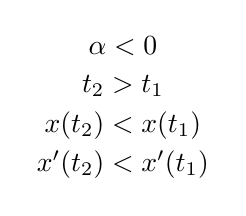
\begin{tikzpicture}
\draw [node distance=0.5cm] (0,0) 
node (a) {$\alpha < 0$} 
node (b) [below of=a] {$t_2>t_1$}
node (c) [below of=b] {$x(t_2)<x(t_1)$}
node [below of=c] {$x^\prime(t_2)<x^\prime(t_1)$};
\end{tikzpicture}

% controls
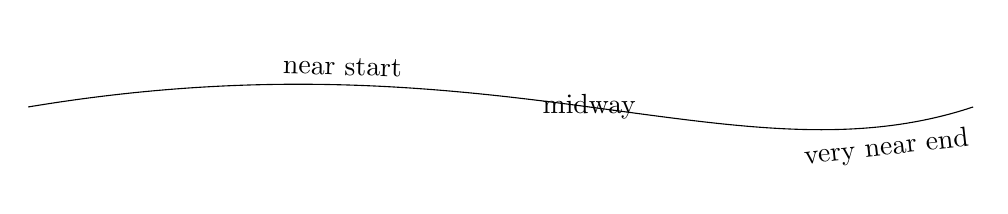
\begin{tikzpicture}
  \draw (0,0) .. controls (6,1) and (9,-1) ..
    node[near start,sloped,above] {near start}
    node {midway}
    node[very near end,sloped,below] {very near end} (12,0);
\end{tikzpicture}


% slope figure
\def\xmax{5}
\def\tmax{6}
\def\tplotmax{4.5}
\def\xmin{-2}
\def\tmin{0}
\def\hang{-0.2}
%
\def\xinit{0.5}
\def\tau{2}
%
\def\tone{2}
\def\xone{\xinit*exp(\tone/\tau)}
\def\slopeone{\xinit*exp(\tone/\tau)/\tau}
%
\def\ttwo{3.5}
\def\xtwo{\xinit*exp(\ttwo/\tau)}
\def\slopetwo{\xinit*exp(\ttwo/\tau)/\tau}
%
\def\base{0.5}
\begin{figure}[t]
\begin{center}
\begin{tikzpicture}[domain=0:4]
    \draw[thick,->] (\hang,0) -- (\tmax,0) node[below left] {$t$};
    \draw[thick,->] (0,\hang) -- (0,\xmax) node[below left] {$x(t)$} node[below right] {$=x_0 e^{\alpha t}$};
\draw[thick, domain=\tmin:\tplotmax,->] plot (\x, { \xinit*exp(\x/\tau) } ) node[below right] {$\alpha > 0$};  
\draw [fill=white] (0,\xinit) node [left] {$x_0$} circle (2pt); 
%
\draw [thick, dotted] (\hang,{\xtwo}) node[left,fill=white] {$x(t_2)$}  -- (\ttwo,{\xtwo}) -- (\ttwo,\hang) node[below] {$t_2$};
\draw [blue, ultra thick,<->]  (\ttwo-\base,{\xtwo-\base*\slopetwo}) -- (\ttwo,{\xtwo}) node [below right,fill=white] {$\mbox{slope} = x^\prime(t_2)$} -- (\ttwo+\base,{\xtwo+\base*\slopetwo}); 
\draw [fill=white] (\ttwo,{\xtwo}) circle (2pt); 
%
\draw [thick, dotted] (\hang,{\xone}) node[left,fill=white] {$x(t_1)$}  -- (\tone,{\xone}) -- (\tone,\hang) node[below] {$t_1$};
\draw [blue, ultra thick,<->]  (\tone-\base,{\xone-\base*\slopeone}) -- (\tone,{\xone}) node [below right,fill=white] {$\mbox{slope} = x^\prime(t_1)$} -- (\tone+\base,{\xone+\base*\slopeone}); 
\draw [fill=white] (\tone,{\xone}) circle (2pt); 
\end{tikzpicture}
\end{center}
\caption{Exponential growth slopes.}
\end{figure}






\def\xmax{4}
\def\tmax{4}
\def\xmin{-2}
\def\tmin{0}
\def\xo{2}
\begin{figure}[h!]
\begin{center}
\begin{tikzpicture}[domain=0:4]
    %\draw[help lines] (-0.1,-0.1) grid (3.9,3.9);
    \draw[thick,->] (-0.2,0) -- (\tmax,0) node[below left] {$t$};
    \draw[thick,->] (0,-0.2) -- (0,\xmax) node[below left] {$x(t)$} node[below right] {$=x_0 e^{\alpha t}$};
    \draw[blue,ultra thick, domain=\tmin:\tmax,->] plot (\x, {\xo*exp(-\x)}) node[above right] {$\alpha < 0$}; 
\draw[blue,ultra thick, domain=\tmin:\tmax,->] plot (\x, {\xo}) node[right] {$\alpha = 0$}; 
\draw[blue,ultra thick, domain=\tmin:3,->] plot (\x, {\xo*exp(\x/5)})  node[below right] {$\alpha > 0$}; 
%\draw[blue,thin, domain=\tmin:1,->] plot (\x, {\xo*exp(\x/2)}); 
%\draw[blue,thin, domain=\tmin:2,->] plot (\x, {\xo*exp(\x/3)}); 
%\draw[blue,thin, domain=\tmin:\tmax,->] plot (\x, {\xo*exp(\x/10)}); 
\draw [fill=white] (0,\xo) node [left] {$x_0$} circle (2pt); 
\end{tikzpicture}
\end{center}
\caption{Caption.}
\end{figure}


% definition of derivative  
\def\xmax{3}
\def\ymax{5}
\def\xmin{-2.25}
\def\ymin{-1}
\begin{figure}
\begin{tikzpicture}
\draw[thick,->] (\xmin,0) -- (\xmax,0) node[below left] {$t$};
\draw[thick,->] (0,\ymin) -- (0,\ymax) node[below left] {$x(t)$};
\draw[blue,ultra thick, domain=\xmin:\xmax,<->] plot (\x, {0.5*(\x)^2});
\foreach \y in { 1.01, 1.2, 1.4, 2, 2.5 } { 
   \draw[thin, blue, domain=1:\xmax,<->] plot (\x,{ 0.5*1^2 + ( 0.5*\y^2 - 0.5*1^2)/(\y - 1)*(\x-1)}); 
   \draw [thick,dotted] (\y,0.5*\y^2) -- (0,0.5*\y^2);
   \draw [thick,dotted] (\y,0) -- (\y,0.5*\y^2);
    };      
\foreach \y in {1.01, 1.2, 1.4, 2, 2.5} { 
     \draw [fill=white] (\y,0.5*\y^2) circle (2pt); 
    };  
\draw[<->]  (1,-0.2) --  node[below] {$\delta t$} (2,-0.2); 
\draw[<->]  (-0.2,0.5*1^2) --  node[left,fill=white] {$\delta x$} (-0.2,0.5*2^2); 
\draw [thick, dotted] (1,0) -- (1,-0.5) node[below] {$\bar{t}$};
\draw [thick, dotted] (2,0) -- (2,-1) node[below] {$\bar{t}+\delta t$};
\draw [thick, dotted] (0,2) -- (-0.5,2) node[left,fill=white] {$x(\bar{t}+\delta t)$};
\draw [thick, dotted] (0,0.5) -- (-0.5,0.5) node[left,fill=white] {$x(\bar{t})$};

\begin{scope}[xshift=6cm]
\draw[thick,->] (\xmin,0) -- (\xmax,0) node[below left] {$t$};
\draw[thick,->] (0,\ymin) -- (0,\ymax) node[below left] {$x^\prime(t)$};
\draw[blue,ultra thick, domain=\xmin:\xmax,<->] plot (\x, \x);
\draw [thick, dotted] (1,1) -- (1,-0.5) node[below] {$\bar{t}$};
\draw [thick, dotted] (1,1) -- (-0.5,1) node[left,fill=white] {$x^\prime(\bar{t})$};
\draw [fill=white] (1,1) circle (2pt); 
\end{scope}
\end{tikzpicture}
\caption{Definition of a derivative}
\end{figure}
 


\begin{figure}
    \tikzstyle{mybox} = [draw=blue, fill=blue!10, very thick,
    rectangle, rounded corners,inner sep=5pt]
\tikzstyle{fancytitle} =[fill=blue, text=white, ellipse]
\begin{center}
\begin{tikzpicture}
\node [mybox] (boxanalytical) { 
     \begin{tikzpicture}
     \node[text width=6cm] {
       \begin{eqnarray}
          f(x) &=& 3x-x^2  \nonumber\\
 f^\prime(x) &=&   3-2x  \nonumber\\[\baselineskip]
  f^\prime(\bar{x}) &=&  3-2\bar{x} = 0  \nonumber\\
\bar{x} &=& \frac{3}{2} = 1\frac{1}{2}  \nonumber
\end{eqnarray}
\[
 f\left(\bar{x}\right) = 3\left( \frac{3}{2} \right)  - \left( \frac{3}{2} \right)^2
= \frac{9}{4}  = 2 \frac{1}{4} 
\]
};
\end{tikzpicture}

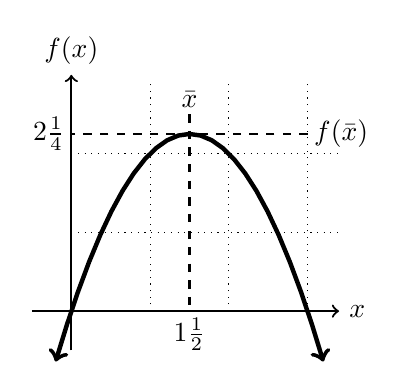
\begin{tikzpicture}
\draw[style=dotted] (0,0) grid (3.4,2.9);
\draw[ultra thick, domain=-0.2:3.2,<->] plot (\x, {-\x*\x +3*\x});
\draw[thick,->] (-0.5,0) -- (3.4,0) node[right] {$x$};
\draw[thick,->] (0,-0.5) -- (0,3.0) node[above] {$f(x)$};
\draw[thick,dashed] (1.5,2.5) node[above,inner sep=2pt] {$\bar{x}$} -- (1.5,0) node[below,inner sep=2pt] {$1\frac{1}{2}$};
\draw[thick,dashed] (3.0,2.25) node[right,inner sep=2pt] {$f(\bar{x})$} -- (0,2.25) node[left,inner sep=2pt] {$2\frac{1}{4}$};
 \end{tikzpicture}
 };
 
 \node[fancytitle] at (boxanalytical.north) {Analytical / Pencil \& Paper};
  
  \node [mybox,below=0.7cm] at (boxanalytical.south) (boxnumerical)  {
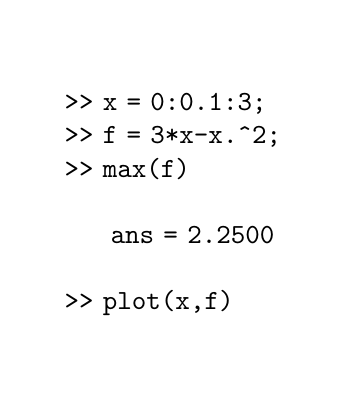
\begin{tikzpicture}[inner sep=10pt]
       \node[text width=3cm] {
   \begin{verbatim}
 >> x = 0:0.1:3;
 >> f = 3*x-x.^2;
 >> max(f)
        
      ans = 2.2500
 
 >> plot(x,f)
 \end{verbatim}
    };
    \end{tikzpicture}
    
    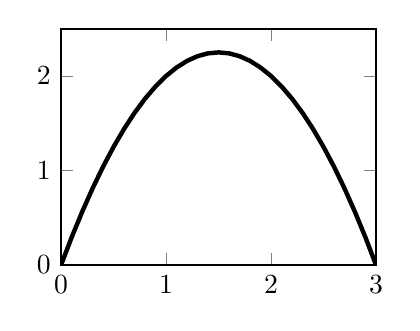
\begin{tikzpicture}
\begin{axis}[%
width=4cm,
height=3cm,
scale only axis,
thick,
xmin=0,
xmax=3,
ymin=0,
ymax=2.5
]
\addplot [
color=black,
solid,
ultra thick,
forget plot
]
table[row sep=crcr]{
0 0\\
0.1 0.29\\
0.2 0.56\\
0.3 0.81\\
0.4 1.04\\
0.5 1.25\\
0.6 1.44\\
0.7 1.61\\
0.8 1.76\\
0.9 1.89\\
1 2\\
1.1 2.09\\
1.2 2.16\\
1.3 2.21\\
1.4 2.24\\
1.5 2.25\\
1.6 2.24\\
1.7 2.21\\
1.8 2.16\\
1.9 2.09\\
2 2\\
2.1 1.89\\
2.2 1.76\\
2.3 1.61\\
2.4 1.44\\
2.5 1.25\\
2.6 1.04\\
2.7 0.81\\
2.8 0.56\\
2.9 0.289999999999999\\
3 0\\
};
\end{axis}
\end{tikzpicture}%
  
        };
  
  \node[fancytitle] at (boxnumerical.north) {Numerical / Computer}; 
  
 \end{tikzpicture}
  \end{center}
  \end{figure}
  
   


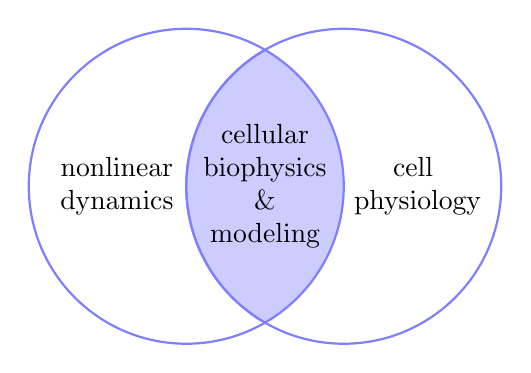
\begin{tikzpicture}
\def\firstcircle{(0,0) circle (2.0cm)}
\def\secondcircle{(0:2cm) circle (2.0cm)}
\colorlet{circle edge}{blue!50}
\colorlet{circle area}{blue!20}
\tikzset{filled/.style={fill=circle area, draw=circle edge, thick},
    outline/.style={draw=circle edge, thick}}
    \begin{scope}
        \clip \firstcircle;
        \fill[filled] \secondcircle;
    \end{scope}
    \draw[outline] \firstcircle node[left, text width=1.5cm,text centered] {nonlinear dynamics};
    \draw[outline] \secondcircle node[right, text width=1.5cm,text centered] {cell\\ physiology};
    \node[text width=2cm,text centered] at (1,0) {cellular\\ biophysics\\ \& \\ modeling};
\end{tikzpicture}




\begin{figure}
\begin{center}
% Define box and box title style
\tikzstyle{mybox} = [draw=red, fill=blue!20, very thick,
    rectangle, rounded corners, inner sep=10pt, inner ysep=20pt]
\tikzstyle{fancytitle} =[fill=red, text=white]

\begin{tikzpicture}
\node [mybox] (box){%
    \begin{minipage}{0.50\textwidth}
        To calculate the horizontal position the kinematic differential
        equations are needed:
        \begin{align}
            \dot{n} &= u\cos\psi -v\sin\psi \\
            \dot{e} &= u\sin\psi + v\cos\psi
        \end{align}
        For small angles the following approximation can be used:
        \begin{align}
            \dot{n} &= u -v\delta_\psi \\
            \dot{e} &= u\delta_\psi + v
        \end{align}
    \end{minipage}
};
\node[fancytitle, right=10pt] at (box.north west) {A fancy title};
\node[fancytitle, rounded corners] at (box.east) {$\clubsuit$};
\end{tikzpicture}%
%
\tikzstyle{mybox} = [draw=blue, fill=green!20, very thick,
    rectangle, rounded corners, inner sep=10pt, inner ysep=20pt]
\tikzstyle{fancytitle} =[fill=blue, text=white, ellipse]
%
\begin{tikzpicture}[transform shape, rotate=10, baseline=-3.5cm]
\node [mybox] (box) {%
    \begin{minipage}[t!]{0.5\textwidth}
        Fermat's Last Theorem states that
        \[
            x^n + y^n = z^n
        \]
        has no non-zero integer solutions for $x$, $y$ and $z$ when $n > 2$.
    \end{minipage}
    };
\node[fancytitle] at (box.north) {Fermat's Last Theorem};
\end{tikzpicture}
\end{center}
\caption{kldfjadls;fjadl;sfj.}
\end{figure}


 Definition of circles
\def\firstcircle{(0,0) circle (1.5cm)}
\def\secondcircle{(0:2cm) circle (1.5cm)}

\colorlet{circle edge}{blue!50}
\colorlet{circle area}{blue!20}

\tikzset{filled/.style={fill=circle area, draw=circle edge, thick},
    outline/.style={draw=circle edge, thick}}

\setlength{\parskip}{5mm}


\begin{tikzpicture}
    \draw[filled, even odd rule] (0,0) circle (2.5cm) node[above] {nonlinear} node[below] {dynamics}
                                 (0:4cm) circle (2.5cm) node[above] {cellular} node[below] {physiology};
    \node[anchor=south] at (current bounding box.north) {Scope of Cellular Biophysics and Modeling};
\end{tikzpicture}

\begin{tikzpicture}
    \draw[filled, even odd rule] (0,0) circle (2.5cm) node {$analytical$}
                                 (0:4cm) circle (2.5cm) node{$numerical$};
    \node[anchor=south] at (current bounding box.north) {$\overline{A \cap B}$};
\end{tikzpicture}


\begin{tikzpicture}
    \begin{scope}
        \firstcircle;
        \fill[filled] \secondcircle;
    \end{scope}
    \draw[outline] \firstcircle node {$analytical$};
    \draw[outline] \secondcircle node {$numerical$};
    \node[anchor=south] at (current bounding box.north) {$A \cap B$};
\end{tikzpicture}



% ORIGINAL STUFF


% Set A and B
\begin{tikzpicture}
    \begin{scope}
        \clip \firstcircle;
        \fill[filled] \secondcircle;
    \end{scope}
    \draw[outline] \firstcircle node {$A$};
    \draw[outline] \secondcircle node {$B$};
    \node[anchor=south] at (current bounding box.north) {$A \cap B$};
\end{tikzpicture}

% characteristic time for changes
\def\xaxismax{4.5}
\def\taxismax{6}
\def\hang{0.2}
%
\def\tplotmin{0}
\def\tplotmax{6}
%
\def\xmax{3.5}
\def\xmin{1}
\def\tstar{\tplotmax/2}
\def\theta{10*\tplotmax}
\def\slope{((\xmax-\xmin)/(\tauchar))}
\def\xmid{(\xmax-\xmin)/2+\xmin}
\def\slopehang{0.5}
%
\def\tauchar{3.14}
\def\tone{\tstar-\tauchar/2}
\def\ttwo{\tstar+\tauchar/2}
%
\begin{figure}[t]
\begin{center}
\begin{tikzpicture}[domain=0:4]
\draw[thick,->] (-\hang,0) -- (\taxismax,0) node[below left] {$t$};
\draw[thick,->] (0,-\hang) -- (0,\xaxismax) node[below left] {$x(t)$} node[below right] {}; 

\draw [thick] (-\hang,\xmax) node[left] {$x_{max}$}  --  (0,\xmax);
\draw [thick, dotted] (0,\xmax) -- (\tplotmax,\xmax); 

\draw [thick] (-\hang,\xmin) node[left] {$x_{min}$}  --  (0,\xmin);
\draw [thick, dotted] (0,\xmin) -- (\tplotmax,\xmin); 

\fill [fill=blue!20,semitransparent]  (\tone,\xmin) -- (\ttwo,\xmax) -- (\ttwo,\xmin) -- cycle; 

\draw [ultra thick,blue,<->]  (\tone,\xmin) -- node[midway,above=1pt,rotate=39,fill=white] {$\mbox{slope} = \max \left| x^\prime(t) \right|$}  (\ttwo,\xmax); 

\draw [thick,|<->|] (\tone,\xmin-0.2)  -- node[below,fill=white] {$\tau_{char}$} (\ttwo,\xmin-0.2) ;

\draw [thick,|<->|] (\ttwo+\hang,\xmin)  -- node[right,fill=white] {$x_{max}-x_{min}$} (\ttwo+\hang,\xmax) ;

\draw[thick, domain=\tplotmin:\tplotmax,samples=200,<->] plot (\x,{ \xmin + (\xmax-\xmin)*(0.5+0.5*tanh((\x-\tstar)/\theta) )   });

\end{tikzpicture}
\end{center}
\caption{Characteristic time for changes in a bounded function.}
\end{figure}

\clearpage
\newpage



\end{document}